\documentclass[10pt]{article}
\usepackage[letterpaper]{geometry}
\geometry{verbose,tmargin=1in,bmargin=1in,lmargin=1in,rmargin=1in}
\usepackage{setspace}
\usepackage{ragged2e}
\usepackage{color}
\usepackage{titlesec}
\usepackage{graphicx}
\usepackage{float}
\usepackage{mathtools}
\usepackage{amsmath}
\usepackage[font=small,labelfont=bf,labelsep=period]{caption}
\usepackage[english]{babel}
\usepackage{indentfirst}
\usepackage{array}
\usepackage{makecell}
\usepackage[usenames,dvipsnames]{xcolor}
\usepackage{multirow}
\usepackage{tabularx}
\usepackage{arydshln}
\usepackage{caption}
\usepackage{subcaption}
\usepackage{xfrac}
\usepackage{etoolbox}
\usepackage{cite}
\usepackage{url}
\usepackage{dcolumn}
\usepackage{hyperref}
\usepackage{courier}
\usepackage{url}
\usepackage{esvect}
\usepackage{commath}
\usepackage{verbatim} % for block comments
\usepackage{enumitem}
\usepackage{hyperref} % for clickable table of contents
\usepackage{braket}
\usepackage{titlesec}
\usepackage{booktabs}
\usepackage{gensymb}
\usepackage{longtable}
\usepackage{listings}
\usepackage{cancel}
\usepackage{tcolorbox}
\usepackage[mathscr]{euscript}
\lstset{
	basicstyle=\ttfamily\small,
    frame=single,
    language=fortran,
    breaklines=true,
    commentstyle=\color{magenta}\ttfamily,
    postbreak=\raisebox{0ex}[0ex][0ex]{\ensuremath{\color{red}\hookrightarrow\space}}
}

% for circled numbers
\usepackage{tikz}
\newcommand*\circled[1]{\tikz[baseline=(char.base)]{
            \node[shape=circle,draw,inner sep=2pt] (char) {#1};}}

\newcommand{\beq}{\begin{equation}}
\newcommand{\eeq}{\end{equation}}
\newcommand{\beqa}{\begin{equation}\begin{aligned}}
\newcommand{\eeqa}{\end{aligned}\end{equation}}

\titleclass{\subsubsubsection}{straight}[\subsection]

% define new command for triple sub sections
\newcounter{subsubsubsection}[subsubsection]
\renewcommand\thesubsubsubsection{\thesubsubsection.\arabic{subsubsubsection}}
\renewcommand\theparagraph{\thesubsubsubsection.\arabic{paragraph}} % optional; useful if paragraphs are to be numbered

\titleformat{\subsubsubsection}
  {\normalfont\normalsize\bfseries}{\thesubsubsubsection}{1em}{}
\titlespacing*{\subsubsubsection}
{0pt}{3.25ex plus 1ex minus .2ex}{1.5ex plus .2ex}

\makeatletter
\renewcommand\paragraph{\@startsection{paragraph}{5}{\z@}%
  {3.25ex \@plus1ex \@minus.2ex}%
  {-1em}%
  {\normalfont\normalsize\bfseries}}
\renewcommand\subparagraph{\@startsection{subparagraph}{6}{\parindent}%
  {3.25ex \@plus1ex \@minus .2ex}%
  {-1em}%
  {\normalfont\normalsize\bfseries}}
\def\toclevel@subsubsubsection{4}
\def\toclevel@paragraph{5}
\def\toclevel@paragraph{6}
\def\l@subsubsubsection{\@dottedtocline{4}{7em}{4em}}
\def\l@paragraph{\@dottedtocline{5}{10em}{5em}}
\def\l@subparagraph{\@dottedtocline{6}{14em}{6em}}
\makeatother

\newcommand{\volume}{\mathop{\ooalign{\hfil$V$\hfil\cr\kern0.08em--\hfil\cr}}\nolimits}

\setcounter{secnumdepth}{4}
\setcounter{tocdepth}{4}

\title{Finite Element Domain Decomposition of the Heat Equation}
\author{April Novak}


\begin{document}
\maketitle

\section{Introduction}

This final project involves the serial creation and parallelization of a finite element (FE) solver to the heat equation, which in its simplest form describes the diffusion of temperature \(T\) with a heat source \(\dot{q}\):

\beq
\label{eq:eq}
-k\frac{\partial^2 T}{\partial x^2}=\dot{q}
\eeq

where \(k\) is the thermal conductivity. While kept simple to allow this project to focus more on parallel algorithms than physics, this equation has very wide areas of applicability. From a nuclear engineering background, this equation describes the temperature distribution in nuclear fuel, which when coupled to neutron transport, can model many of the most important features of a nuclear reactor. This equation will be solved using domain decomposition (DD) methods in 1-D using MPI for controlling the coarse-grained DD algorithm. While application of DD to this equation is not new, I chose this topic because DD is one of the most well-established methods for parallel solutions to PDEs, and appears in my research using FE methods for fluid dynamics simulations.

Due to the second derivative present, two boundary conditions are needed (one on each end of the 1-D domain). This presents the fundamental difficulty of parallelizing a DD solution - if the domain is divided amongst different parallel processes, then the equations cannot be solved unless guesses are made for the conditions on the interface boundaries that are created upon decomposition (for the purposes of this report, ``interface'' is defined as the nodes that are shared by more than one domain). But the solution is not known {\t a priori}, so any DD solution will require an iterative method, where an initial guess for the interface boundary conditions is continually improved until all domains ``agree'' on the values at the interface locations. DD is \textit{not} embarrassingly parallel, and if the number of iterations required to converge to the true global solution is very large, then the parallel runtime can easily be longer than the serial runtime. This interesting feature was not present in any of our homework assignments - while parallel code in homeworks could be slower due to communication overhead than the serial code, adding {\it iterations} places a stricter constraint on the success of a parallel algorithm. Much effort was devoted in this project to means by which the number of parallel iterations could be reduced to make DD a viable method.

\section{The Finite Element Method}
This section discusses the FEM applied to the heat equation in 1-D. I have chosen the FEM as the PDE solver because my research uses the Multiphysics Object Oriented Simulation Environment (MOOSE) developed by Idaho National Laboratory to solve problems in nuclear engineering. With a field so tightly export-controlled, the nuclear industry has to develop it's own set of modeling tools that will never be able to be incorporated into commercial software such as COMSOL.

Some familiarity with numerical methods is assumed so that the brunt of this report can focus on parallelization. A large fraction of the discussion of the numerical method is deferred to the Appendix, and only the elements necessary to understand the parallel implementation are discussed here (feel free to skip the Appendix). The FEM is a weighted residual method that solves the weak form of the governing equation. The weak form is obtained by multiplying Eq. \eqref{eq:eq} by a test function \(\psi(x)\) and integrating over all space:

\beq
\int_{\Omega}\frac{\partial T}{\partial x}k\frac{\partial\psi(x)}{\partial x}dx-\int_{\Gamma}k\frac{\partial T}{\partial x}\psi(x)\cdot\hat{n}dx=\int_{\Omega}\dot{q}\psi(x)dx
\eeq

where \(\Omega\) indicates the entire domain and \(\Gamma\) its boundary. Now, we assume that the numerical solution \(T_h\) is a sum of coefficients multiplied by expansion functions \(\phi\):

\beq
T_h=\sum_{j=1}^{N}c_j\phi_j(x)
\eeq

where there are \(N\) of these expansion functions defined over the domain. The numerical method reduces to the problem of determining the expansion coefficients \(c_j\) for a user-selected set of \(\phi_j(x)\). The Galerkin FEM specifies that \(\psi\) should come from the same space as \(T_h\). Hence, inserting these expansions into the weak form gives a discrete set of matrix equations that can be solved:

\beq
K_{ij}c_j=R_i
\eeq

where the stiffness matrix is:

\beq
\label{eq:k}
K_{ij}=\int_{\Omega}\frac{\partial \phi_j(x)}{\partial x}k\frac{\partial\phi_i(x)}{\partial x}dx-\int_{\Gamma}k\frac{\partial \phi_j(x)}{\partial x}\phi_i(x)\cdot\hat{n}dx
\eeq

and the load vector is:

\beq
R_{i}=\int_{\Omega}\dot{q}\phi_i(x)dx
\eeq

In order to solve this discrete system, it is much easier to solve the system over each element individually and then assemble the local information together into a single, large, matrix system. 

\(K_{ij}\) shown in Eq. \eqref{eq:k} consists of the multiplication of the derivatives of \(\phi_i(x)\) with \(\phi_j(x)\). If these shape functions are defined over the {\it entire} domain, then \(K_{ij}\) will be dense (not an advantage from either memory or flops). If we choose these shape functions to be nonzero only over a single small region of the domain instead, then the product of cross terms will be zero for most of the matrix, giving a sparse matrix. The matrix equation \(K_{ij}c_j=R_i\) can be written for each individual element as \(K_{ij}^ec_j^e=R_i^e\), with a post-processing step that takes the system of equations for each element and connects them all together to enforce solution continuity at element interfaces. 

\beq
K_{ij}^e=\int_{\Omega^e}\frac{\partial \phi_j(x)}{\partial x}k\frac{\partial\phi_i(x)}{\partial x}dx-\int_{\Gamma^e}k\frac{\partial \phi_j(x)}{\partial x}\phi_i(x)\cdot\hat{n}dx
\eeq

\beq
R_{i}^e=\int_{\Omega^e}\dot{q}\phi_i(x)dx
\eeq

The system of equations for each element cannot be solved independently of the other elements since we require solution continuity at inter-element nodes. This requires the formation of a connectivity matrix. A connectivity matrix is used to describe how the local element nodes map into the global system. Figure \ref{fig:FEmesh} shows a simple FE mesh, where the numbers illustrate the global node numbering. A location matrix is required to map from the elemental perspective to this global mesh. 

\begin{figure}[H]
\centering
\includegraphics[width=0.6\textwidth]{../figures/FEmesh.pdf}
\caption{Global node numbering in a simple FE mesh. Source:\newline {\tt http://opensees.berkeley.edu/wiki/index.php/}\newline{\tt Simply\_supported\_beam\_modeled\_with\_two\_dimensional\_solid\_elements}}
\label{fig:FEmesh}
\end{figure}

Each column of the location matrix corresponds to one element, and gives the global node numbers that correspond to the local node numbers. The first five columns of the location matrix for this mesh would be:

\beq
\label{eq:LM}
LM=\begin{bmatrix}
1 & 2 & 3 & 4 & 5 & \cdots\\
2 & 3 & 4 & 5 & 6 & \cdots\\
11 & 12 & 13 & 14 & 15 & \cdots\\
10 & 11 & 12 & 13 & 14 & \cdots\\
\end{bmatrix}
\eeq

where the nodes have been numbered counterclockwise. Once this location matrix is known, the elemental system of equations can be assembled into the global system of equations. For illustration, several entries of \textbf{K} are assembled as follows for the location matrix given in Eq. \eqref{eq:LM}. The important thing to note here is that the formation of the global matrix is {\it additive}, in that there is not a one-to-one correspondence of entries in the location matrix to those in the global matrix (entries overlap). 

\beqa
K(1, 1) =& k(1, 1)^{e=1}\\
K(1, 2) =& k(1, 2)^{e=1}\\
K(2, 2) =& k(2, 2)^{e=1}+k(1, 1)^{e=2}\\
K(2, 11) =& k(2, 3)^{e=1}\\
K(12, 12) =& k(3, 3)^{e=2}+k(4, 4)^{e=3}\\
\eeqa

where a new notation of lowercase \(k\) representing \(K^e\) is used. \(e\) superscripts give the element numbers corresponding to the entries of the local stiffness matrix \(k\). Any Dirichlet boundary conditions must now be applied within the matrix system (Neumann boundary conditions have naturally been applied by the form of the perimeter integral in Eq. \eqref{eq:k}) by ``removing'' Dirichlet nodes from the solve. For a 1-D domain consisting of three linear elements (two nodes per element), the global matrix system \(\textbf{K}c=\textbf{R}\) before imposition of Dirichlet boundary conditions is:

\beq
\begin{bmatrix}
k(1, 1)^{e=1} & k(1, 2)^{e=1} & 0 & 0\\
k(2, 1)^{e=1} & k(2, 2)^{e=1}+k(1, 1)^{e=2} & k(1, 2)^{e=2} & 0\\
0 & k(2, 1)^{e=2} & k(2, 2)^{e=2}+k(1, 1)^{e=3} & k(1, 2)^{e=3}\\
0 & 0 & k(2, 1)^{e=3} & k(2, 2)^{e=3}\\
\end{bmatrix}
\begin{bmatrix}
c_1\\c_2\\c_3\\c_4
\end{bmatrix}
=\begin{bmatrix}
r(1)^{e=1} \\ r(2)^{e=1}+r(1)^{e=2}\\r(2)^{e=2}+r(1)^{e=3}\\r(2)^{e=3}\\
\end{bmatrix}
\eeq

To apply Dirichlet boundary conditions at nodes \(1\) and \(4\), in rows 1 and 4, the off-diagonal terms are set to zero and the on-diagonal terms to unity. For instance, to impose Dirichlet conditions of \(T(\textrm{node} 1)=3.5\) and \(T(\textrm{node} 5) = 10.5\), the global matrix system becomes:

\beq
\begin{bmatrix}
1 & 0 & 0 & 0\\
k(2, 1)^{e=1} & k(2, 2)^{e=1}+k(1, 1)^{e=2} & k(1, 2)^{e=2} & 0\\
0 & k(2, 1)^{e=2} & k(2, 2)^{e=2}+k(1, 1)^{e=3} & k(1, 2)^{e=3}\\
0 & 0 & 0 & 1\\
\end{bmatrix}
\begin{bmatrix}
c_1\\c_2\\c_3\\c_4
\end{bmatrix}
=\begin{bmatrix}
3.5\\ r(2)^{e=1}+r(1)^{e=2}\\r(2)^{e=2}+r(1)^{e=3}\\10.5\\
\end{bmatrix}
\eeq

Then, the matrix system can be solved by your favorite linear algebra routine. For this assignment, the Conjugate Gradient (CG) method is selected to solve this symmetric system. To solve a matrix system \(\textbf{K}a=R\) by the CG method requires rewriting the governing equation as the minimization of a potential \(\Pi\). The exact solution is obtained by taking the gradient of this potential with respect to each of the expansion coefficients in the solution vector and setting that gradient equal to zero. The CG method requires computation of the residual:

\beq
r^i=R-\textbf{K}a^i
\eeq

where \(i\) is the iteration index. Each update to the solution iterates is performed according to Eq. \eqref{eq:CGUpdate}, where the update scales by \(z^i\) as shown in Eq. \eqref{eq:ZUpdateCG}.

\beq
\label{eq:CGUpdate}
a^{i+1}=a^i+\lambda^iz^i
\eeq

\beq
\label{eq:ZUpdateCG}
z^i=r^i+\theta^iz^{i-1}
\eeq

\(\theta^i\) is a parameter chosen such that \(z^i\) is \(\textbf{K}\)-conjugate to \(z^{i-1}\), or:

\beq
\label{eq:kconjugate}
z^{T,i}\textbf{K}z^{i-1}=0
\eeq

In other words, the search direction is a combination of a move in the reverse direction of the gradient (method of steepest descent) plus a motion perpendicular to that direction. This helps to avoid duplicate searching in the same general area. For the very first iteration, it is common to select \(z^1=r^1\). Plugging in Eq. \eqref{eq:ZUpdateCG} to Eq. \eqref{eq:kconjugate} gives:

\beq
\theta^i=-\frac{r^{T,i}\textbf{K}z^{i-1}}{z^{T,i-1}\textbf{K}z^{i-1}}
\eeq

Plugging in Eq. \eqref{eq:CGUpdate} into the potential function and taking the partial derivative with respect to \(\lambda^i\), the optimal \(\lambda^i\) is:

\beq
\label{eq:UpdateCG}
\lambda^i=\frac{z^{T,i}r^i}{z^{T,i}\textbf{K}z^i}
\eeq

This concludes the theoretical discussion of the FEM applied to this simple 1-D heat equation. The next section discusses steps taken to obtain a fast serial implementation of this algorithm, and will go into more detail regarding exactly how this method can be implemented. Although the heat equation is only solved in 1-D, no shortcuts are taken with the development of the code. That is, I assume nothing about the structure of the matrices or boundary conditions that would invalidate natural extension to higher dimensions.

\section{Serial Implementation}

This section discusses the serial code that is used as a launching point for parallelization. As a nuclear engineering student interested in computational methods, you will quickly learn that the consequences of errors in codes used to design nuclear reactors can potentially be very high. Hence, in this field there is very slow acceptance of new modeling codes since each new code must undergo rigorous verification and validation. Many nuclear simulation codes are written in Fortran, so I used this project as an opportunity to learn how to program in modern Fortran. Psuedo-code for the overall serial program structure is as follows:

\begin{lstlisting}
! read in problem parameters from command line and namelist
call read_namelist(); call read_commandline()

! initialize problem variables based on user inputs
call initialize_global_mesh(); call define_quadset(); call define_shapefunctions()

! determine elemental matrices
call elementalload(); call elementalstiffness()

! find a good initial guess to serve as input to the CG solver (discussed later)

! form location matrix
LMfine = locationmatrix(global%n_el, global%n_nodes)

! form global load vector and apply boundary conditions
global%rglob  = globalvector(LMfine, rel, global%n_nodes)

! determine CSR storage of global stiffness matrix
call form_csr(LMfine, global%n_nodes, rows)

! call CG method to solve
solution = conjugategradient(rows, guess, global%rglob, global%BCs)
\end{lstlisting}

Every problem begins by initializing problem variables and determining the elemental matrices. An initial guess is required for the CG solver, and can be as naive as a vector of zeros, or determined in a more fancy way (to be discussed later). Then, the global load vector is formed by looping through the connectivity matrix. The global stiffness matrix is stored in Compressed Sparse Row (CSR) format, to be discussed in the next section. Finally, the CG method is called with the initial guess and the {\tt rows} data structure holding the CSR information. After reaching a specified convergence tolerance in the CG solver, the solution is written to a text file for plotting.

\subsection{CSR Format}
An important improvement above code that I've written for FE classes in the past is the storage of the global stiffness matrix in CSR form. The global stiffness matrix is sparse because we select shape functions that are local to an element (they don't extend over the entire physical domain). With linear elements in 1-D, a maximum of \(4N\) non-zero entries would need to be stored (with \(N\) the number of elements), though naive implementations would store all \(N^2\) numbers. Because we only every need the product of the stiffness matrix with a vector, we don't need to store these zeros. CSR storage has about \(\mathscr{O}(N)\) less storage requirements than a naive implementation. The difficulty with implementing CSR storage here is that the structure of the matrix is not known until you actually form the matrix, because there is not a one-to-one correspondence of entries in local matrices to entries in global matrices. That is, some entries overlap due to continuity requirements at inter-element nodes. For instance, in 1-D with linear elements, each element contributes four non-zero numbers to the global stiffness matrix. However, due to continuity, some entries will overlap (they are added), and the global matrix will only have \(3N-2\) nonzero entries. So how can we use the information in the connectivity matrix to determine which entries of the global matrix result due to a single number and how many result due to summations of several contributions?

To form the CSR for this application, we need to determine a relationship between the number of times a node number appears in the connectivity matrix with how many nonzero entries appear on that row in the global matrix. This relationship is different depending on the dimension of the mesh and type of element. For 1-D elements, if a node number appears \(n\) times in the connectivity matrix, then that row in the global matrix has \(2(n-1)\) nonzero entries. The CSR storage is formed by looping over the connectivity matrix and counting the number of times each node number appears, and then saving the nonzero values in a vector, and the column numbers corresponding to those nonzero values (which are the entries of the location matrix for that element) in a vector. The difference between the CSR implementation in this project and that discussed in lecture is that there are multiple entries in the ``columns'' array for a particular row. For illustration, consider the following global stiffness matrix, where summations are shown explicitly in the matrix to illustrate how the number of nonzero entries in a row does not necessarily equal how many ``values'' appear (i.e. row two has three nonzero values, but {\it four} numbers contributed to them):

\beq
K=\begin{bmatrix}
1 & -1 & 0 & 0 & 0\\
-1 & 1 + 1 & -1 & 0 & 0\\
0 & -1 & 1 + 1 & -1 & 0\\
0 & 0 & -1 & 1 + 1 & -1\\
0 & 0 & 0 & -1 & 1\\
\end{bmatrix}
\eeq

As implemented, the CSR format is stored as an array of data type {\tt row}, where {\tt row} consists of two vectors, {\tt values} to hold the numeric values, and {\tt columns} to hold the column numbers. The second row of the above matrix is stored as {\tt my\_matrix(2)\%values = (/-1, 1, 1, -1/)} and the columns as {\tt my\_matrix(2)\%columns = (/1, 2, 2, 3/)}. The runtime associated with this data structure formation is negligible, being less than 0.1\%. 

\subsection{Vectorization}
Single Instruction, Multiple Data (SIMD) is the process by which a single instruction is used to perform an operation on multiple pieces of data at the same time within a single core. When instructed with the appropriate vectorization flags, the compiler will try to find as much SIMD parallelism as possible while being conservative. For all timing results shown, using the {\tt -O3} flag gives dramatic performance improvements. The great performance (in addition to memory) benefit of the CSR storage is not fully appreciated without an understanding of why some loops cannot be automatically vectorized. If we wanted to avoid the CSR implementation, but still only store the nonzero values of the sparse stiffness matrix, we could implement a different algorithm for sparse matrix-vector multiplication. This requires looping over the location matrix {\it during} multiplication, as shown below. Because it is not known {\it which} nodes contribute to the overlapping nodes in the global matrix a priori, this algorithm cannot be vectorized, again due to loop dependence. {\it And}, due to Amdahl's law, this would have a major impact, since matrix-vector multiplication is the fundamental computing paradigm that appears in the CG solver, which accounts for about 99\% of the total runtime.

\begin{lstlisting}
result = 0.0
do q = 1, n_el ! loop over the elements
  do i = 1, n_en ! loop over all entries in vector
      do j = 1, n_en ! loop over all entries in vector
        ! loop cannot be vectorized
        result(LM(i, q)) = result(LM(i, q)) + matrix(i, j) * vector(LM(j, q))
      end do
  end do
end do
\end{lstlisting}


\subsection{Conjugate Gradient Scaling}
Because the cost of a matrix-vector product is roughly \(\mathscr{O}(N)\), the cost of the CG solver is \(I\mathscr{O}(n)\), where \(I\) is the number of CG iterations required. However, timing studies show that this routine scales as \(\mathscr{O}(N^2)\), where \(N\) is the size of the matrix. This can be explained by the fact that the CG method is technically a direct method once you perform \(N\) iterations. So, without good preconditioning, the CG method will scale as \(\mathscr{O}(N^2)\). For lack of time, no preconditioning is used in this assignment. About 99.9\% of the runtime is spent in the CG solver for the serial implementation, which has a dramatic impact on the parallel performance using DD. Suppose a domain of \(N\) elements is subdivided into \(m\) decomposed domains, where an MPI process will solve one \(m\)-sized domain. The speedup is approximately:

\beq
\textrm{Speedup}=\frac{N^2}{(N/m)^2}=m^2
\eeq

Hence, theoretically (provided the communication costs don't dominate the parallel algorithm), the speedup will be {\it greater} than linear - the parallel performance will continually improve with higher numbers of parallel processes! 


\section{Parallel Implementation}
This section discusses parallelization of the serial algorithm. In general, there are two very different parallelization strategies here - the first involves DD amongst parallel processes, where each parallel process then runs a complete FEM solution, with iteration between threads until all threads agree on the values of the solution at the interfaces. Alternatively, a single FEM problem can be run (with no need to iterate boundary conditions because the domain is not decomposed), and the work for the single FEM solve distributed amongst parallel instances. The problem with this second method is that the iterative solution occurs with a {\tt do while} loop. This limits the overall CG solver to effectively serial implementation (a future iteration cannot be done at the same time as an earlier iteration because they are not independent), so DD is more effective. In addition, because the CG method scales as \(\mathscr{O}(N^2)\) (without good preconditioning), the resulting smaller matrix systems formed will lead to quadratic speedup. DD is also useful because the domain may be so large and the problem information so large that it cannot fit into the memory of a single processor. 

There are many variants of DD algorithms, the earliest being Schwarz methods developed to verify analytical solutions to differential equations on strange-shaped domains that could be decomposed into simpler shapes. It appears that most DD methods can be divided into two general categories:

\begin{enumerate}
\item Classes with no ``interface'' problem. In this case, the decomposed domains {\it overlap}. The first DD method developed by Schwarz falls into this category. Half of the domains solve their domain, using initial guesses for the internal boundary conditions. Then, because the domains overlap, the first half of the domains send a boundary condition value to the second half of domains (indicated with downward blue arrows), which then solve over their domains individually. This second group then passes updated boundary condition values back to the first group (indicated with upward blue arrows), and iteration continues until convergence. 

\begin{figure}[H]
\centering
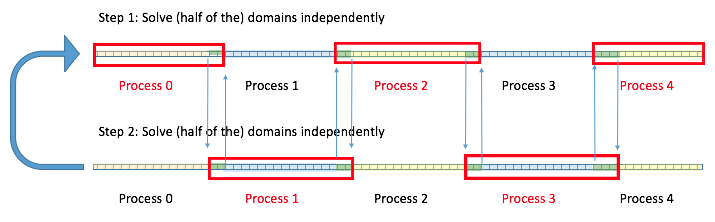
\includegraphics[width=0.8\textwidth]{../figures/1D-schwarz2.png}
\caption{Basic algorithm for 1-D domain decomposition using the Schwarz method.}
\end{figure}

\item Classes that solve an ``interface'' problem. In this case, the decomposed domains do {\it not} overlap. All locations where boundary conditions are imposed are indicated with vertical red lines below. Because the solution is not known a-priori, the boundary conditions at the interfaces must be initially guessed. After each process solves its domain, an interface problem is solved between each domain using updated solution values from the most recent domain solve. The interface problem is used to compute an updated interface boundary condition, which is sent back to the individual domains. Iteration continues until convergence.

\begin{figure}[H]
\centering
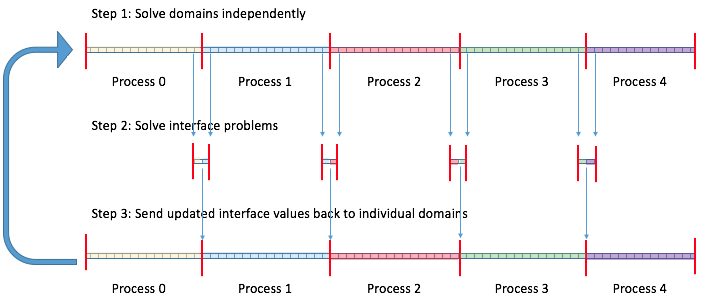
\includegraphics[width=0.8\textwidth]{../figures/1D-dd2.png}
\caption{Basic algorithm for 1-D domain decomposition using the interface problem method.}
\end{figure}

There are several possible algorithms for solving the interface problem. A master-slave approach uses a single process to compute all interface problems. This is the natural approach in higher dimensions when the interfaces between the domains are connected (like the white regions on giraffe skin). However, in 1-D, an alternative approach has each process communicate a single boundary condition value to its right neighbor. Then, each process (except rank 0) solves an interface problem and communicates a single value back to its left neighbor. This approach can only be used when the interfaces are decoupled from each other, but offers greater potential for parallel efficiency since at most one process is idle during the interface solve (as opposed to \(P-1\) idle with the master-slave approach). In higher dimensions, the master-slave approach does not necessarily need to be used, and recursive DD could be applied to solve the interface problem using multiple MPI processes.
\end{enumerate}

The interface problem method, where each domain communicates with at most two other domains (its left and right neighbors), is pursued in this project. This reduces the number of broadcast operations required and also has the potential to reduce overall runtime because each processor at most communicates with two other processors and only one process is idle during the interface solve. 

Extra pre-processing steps are necessary to divide the domain into as-close-as-possible equal-sized domains and prescribe initial guesses for the interface boundary conditions. Then, in a {\tt while} loop, the processes solve their domains individually. Each process (except rank \(P-1\)) sends an updated boundary condition to their right neighbor. Each process (except rank 0) receives this value, computes an interface solution, and sends an updated boundary condition to their left neighbor. The following pseudo code shows the MPI implementation of this algorithm. Because the Poisson equation transmits information at infinite speeds, convergence of the DD algorithm fundamentally has to be based on the errors computed at {\it all} interfaces. That is, a process cannot finish in less iterations than some other process, since the problem is inherently global. Hence, a barrier is required before beginning the next iteration loop. A DD iteration tolerance of 0.00001 is used for all results shown.

\begin{lstlisting}
! divide problem into domains and assign to processes ...

do while (iteration_error > tolerance) ! iteration loop 
  ! save the previous values of the interface BCs
  prev = dd(rank)%BCvals

  ! each processor solves for its domain --------------------------------------
  ! apply updated boundary conditions
  dd(rank)%rglob(dd(rank)%BCs(1)) = dd(rank)%BCvals(1)
  dd(rank)%rglob(dd(rank)%BCs(2)) = dd(rank)%BCvals(2)

  dd(rank)%a = conjugategradient(rows, dd(rank)%a, dd(rank)%rglob, dd(rank)%BCs)

  ! each processor sends a boundary value to the processor to the right -------
  if (rank /= numprocs - 1) then
    call mpi_send(dd(rank)%a(dd(rank)%n_nodes - 1), 1, mpi_real8, rank + 1, rank, ...)
  end if

  ! processor to the right receives the message -------------------------------
  if (rank /= 0) then
    call mpi_recv(BClocals(1), 1, mpi_real8, rank - 1, rank - 1, ...)
    BClocals(2) = dd(rank)%a(2)
  end if

  call mpi_barrier(mpi_comm_world, ierr)

  ! each process solves its interface problem and sends to rank - 1 ---------
  if (rank /= 0) then
    dd(rank)%BCvals(1) = (rel(2) + rel(1) - kel(2, 1) * BClocals(2) &
                      - kel(1, 2) * BClocals(1)) / (kel(2, 2) + kel(1, 1))
    call mpi_send(dd(rank)%BCvals(1), 1, mpi_real8, rank - 1, rank, ...)
  end if

  ! rank - 1 process receives from the process to the right -------------------
  if (rank /= numprocs - 1) then
    call mpi_recv(dd(rank)%BCvals(2), 1, mpi_real8, rank + 1, rank + 1, ...)
  end if

  ! compute iteration error to determine whether to continue looping ----------
  call mpi_allreduce(abs(dd(rank)%BCvals - prev), iteration_error, 1, mpi_real8, &
                                mpi_sum, mpi_comm_world, ierr)

  call mpi_barrier(mpi_comm_world, ierr)
  ddcnt = ddcnt + 1
end do ! ends outermost domain decomposition loop
\end{lstlisting}

The pre-processing step of computing DD information such as the domain edge points and initial boundary condition values are computed (redundantly) by {\it every} MPI process. This eliminates communication from a single process to all other processes of this information, which would be more costly than simply having every process recompute the same information. The cost of the DD algorithm scales as \(D\mathscr{O}(N/m)^2\), where \(D\) is the total number of DD iterations and \(m\) the number of processes (since the cost of the serial algorithm scales as \(\mathscr{O}(N^2)\). Hence, the parallel speedup is:

\beq
\textrm{Speedup}=\frac{N^2}{D(N/m)^2}=\frac{m^2}{D}
\eeq

To be successful, the parallel implementation must converge in less that \(m^2\) DD iterations. The solution over the domain, given a constant heat source and thermal conductivity, will be parabolic. But, assuming we don't know this information, an initial guess for the interface boundary conditions was selected by assuming a straight-line solution between the two endpoints. Iterative global solutions are plotted in Fig. \ref{fig:interface}(a) for four MPI processes for an interface width of two elements (i.e. each interface problem solves a 2-element domain, centered on the interface boundary between the decomposed domains). Each dashed line represents a DD iteration (where interface BCs are updated between each iteration), with only every {\it 20} iterations shown. With this initial boundary condition guess, 1017 DD iterations are required, which is substantially more than our limit of \(5^2=25\). 

The first approach taken to reduce the total number of DD iterations was to used a wider interface problem (i.e. increase the white-skinned section of giraffe skin). That is, the width of each domain stays the same, but the interface regions becomes wider. This leads to faster convergence because the solution will change in proportion to the difference in the boundary conditions at the edges of the interface region. Results obtained for the same problem with an interface width of 10 elements is shown in Fig. \ref{fig:interface}(b). With this wider interface, only 234 DD iterations are required (still too many), but the solution obtained is now incorrect! The larger the interface, the greater the magnitude of the {\it error} in the initial boundary condition guesses (because the straight-line solution is incorrect), and choosing a wider interface applies this error over a wider range. For this particular example, this results in a sharp corner developing in the solution. This interesting result shows that the interface region must be kept very small, which does not help solve the too-many-DD-iterations problem.

\begin{figure}[H]
        \centering
        \begin{subfigure}[b]{0.5\textwidth}
                \centering
                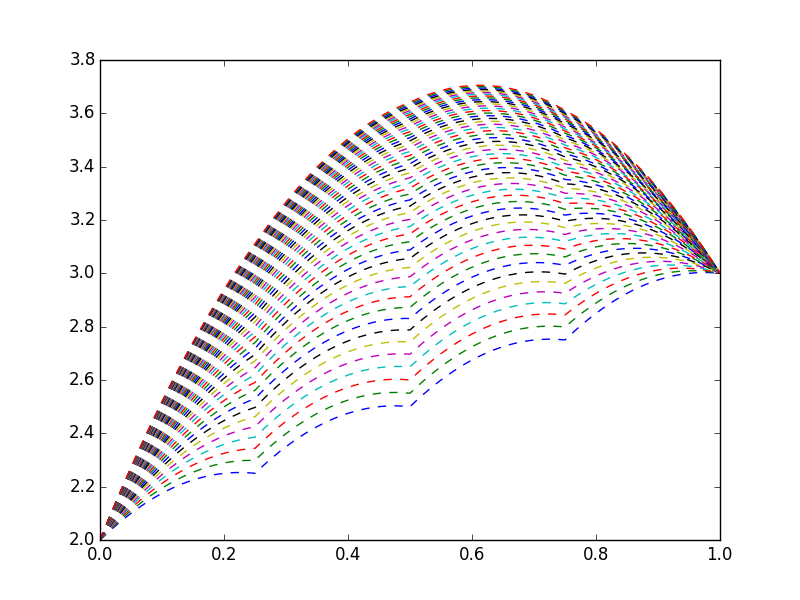
\includegraphics[width=\textwidth]{../figures/interface1.png}
                \caption{Interface width of 2 elements}
        \end{subfigure}%
                \begin{subfigure}[b]{0.5\textwidth}
                \centering
                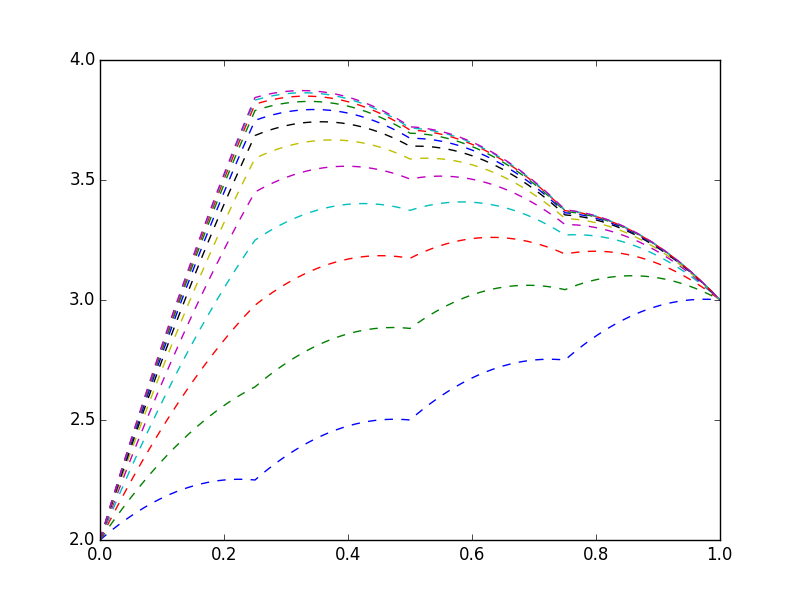
\includegraphics[width=\textwidth]{../figures/interface2.png}
                \caption{Interface width of 10 elements}
        \end{subfigure}%
        \caption{Iterative solutions (only every 20 iterations are plotted) for an interface width of (a) 2 elements and (b) 10 elements for four MPI processes, 500 elements, and initial interface boundary condition values given by a straight line between the two endpoints.}
\label{fig:interface}
\end{figure}

The next approach taken to reduce the number of DD iterations was to improve the initial boundary conditions guesses by solving a coarse-mesh problem. For a five-process solve, the coarse mesh would consist of five elements, with nodes at the same locations as the domain interfaces. After the rank 0 process computes this solution (the algorithm for which is identical to the larger solves, but with fewer elements), the better interface initial conditions are broadcast to all other processes, and then every process continues with the DD algorithm described earlier. This change produced a {\it huge} improvement. For the same iteration tolerance, only one DD iteration is required! Hence, a major take-away from this project is that parallel implementations that require iteration amongst processes can easily be fundamentally slower than serial implementations (not just because of communication overhead, but rather the introduction of an iterative algorithm into a serial code that did not require such iteration), even if {\it theoretically} they should be faster because the ODE solver scales as \(\mathscr{O}(N^2)\). For this project, the use of this better inter-processor initial condition was used to yield a successful implementation. In practice, many codes that use DD will perform a coarse mesh solution that is also used for preconditioning to further enhance the parallel viability of an iterative DD method.

\section{Implementation Results}
This section discusses implementation results obtained once parallelizing using MPI. To keep comparisons fair, the serial cases use the same initial conditions as the MPI cases. A number of ``pseudo processes'' are passed on the command line to the serial case to compute the coarse mesh initial conditions (which is input as an initial guess to the CG solver). When using the same initial condition, the serial and parallel implementations perform the same number of cumulative CG iterations (because with the better initial condition only one DD iteration is needed). The only difference is that for the parallel implementations, each process performs a subset of the iterations. All results are obtained on Edison.

Fig. \ref{fig:speedupMPI} shows the speedup as a function of the number of MPI processes for a single node with 20,000 elements. The speedup is computed as the serial runtime to the parallel runtime for the given number of MPI processes. Because the speedup scales as \(m^2/D\), and only one DD iteration occurs for this test, the speedup is shown in (b) scaled by \(m^2\). Scaling by \(m^2\) changes quadratic speedup behavior to linear in order to illustrate the efficiency of the parallel algorithm {\it independent} of the scaling benefit awarded by the algorithm selection. As can be seen, although the speedup is very large, there is still a lot of room for improvement in the parallel algorithm, since the speedup, scaled by \(m^2\) appears to decrease linearly. This decreasing trend could indicate that my estimates for cost are overly simplified (in which case scaling by \(m^2\) is meaningless), on the other hand. In terms of the absolute speedup, there is no ``optimal'' number of MPI processes per node, since the greater the number, the greater the performance. However, from (b) below, it would appear that 3 MPI tasks per node would be optimal, since this combines a speedup of about 40 before the large drop in speedup when normalized (again assuming scaling by \(m^2\) is meaningful). 

\begin{figure}[H]
        \centering
        \begin{subfigure}[b]{0.5\textwidth}
                \centering
                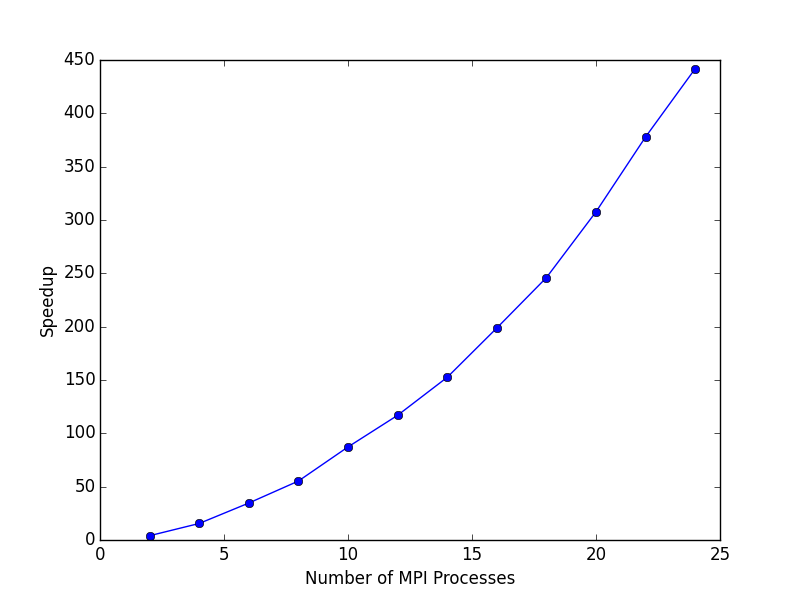
\includegraphics[width=\textwidth]{../figures/unscaled-mpi.png}
                \caption{Raw}
        \end{subfigure}%
                \begin{subfigure}[b]{0.5\textwidth}
                \centering
                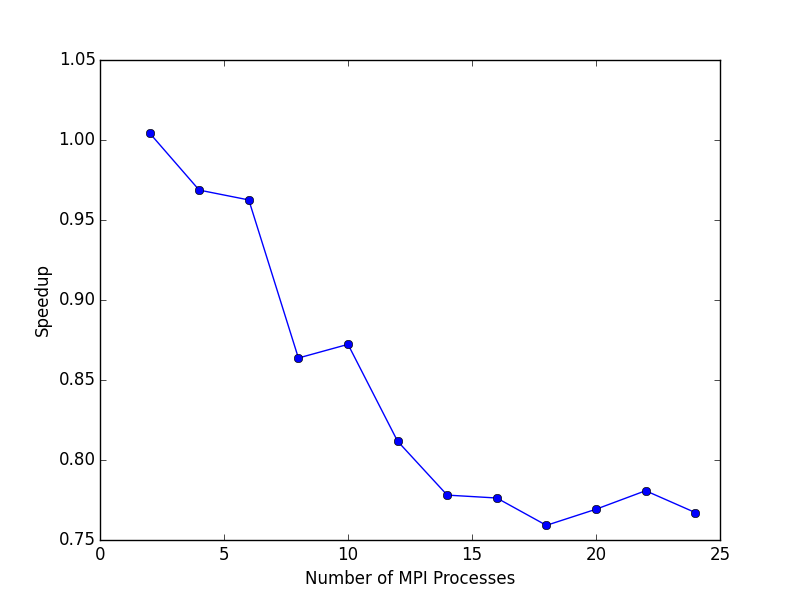
\includegraphics[width=\textwidth]{../figures/scaled-mpi.png}
                \caption{Scaled by \(m^2\)}
        \end{subfigure}%
\caption{Runtime as a function of the number of MPI processes on a single node for 20,000 elements. Plot (b) shows the same speedup, scaled by \(m^2\), where \(m\) is the number of MPI processes.}
        \label{fig:speedupMPI}
\end{figure}

To estimate the runtime consumed by communication between MPI Processes, the very good coarse mesh initial guess is removed (such that the number of DD iterations again becomes large). Previously, the good initial guess gives only one DD iteration, which is not statistically useful for estimating communication. For 5,000 elements and the poor initial guess, roughly \(mN\) DD iterations are performed, where \(m\) is the number of MPI processes and \(N\) the number of elements. All communication within the DD loop can be removed (which will of course give incorrect results) but the number of DD loop iterations set equal to the number required with correct communications in order to evaluate the fraction of runtime that is spent in MPI communications. A switch-case statement is inserted into the code to select the exact same number of DD iterations as the unmodified code to obtain as-fair-as-possible comparison. Then, all communications within the DD loop are commented out, and the same tests run. Fig. \ref{fig:nocomm} shows the decrease in runtime once the communication is removed. As can be seen, communication accounts for roughly half of the runtime of the DD algorithm. However, this communication cannot be entirely removed, or else the domains would solve independently, and would not obtain the correct solution. 

\begin{figure}[H]
\centering
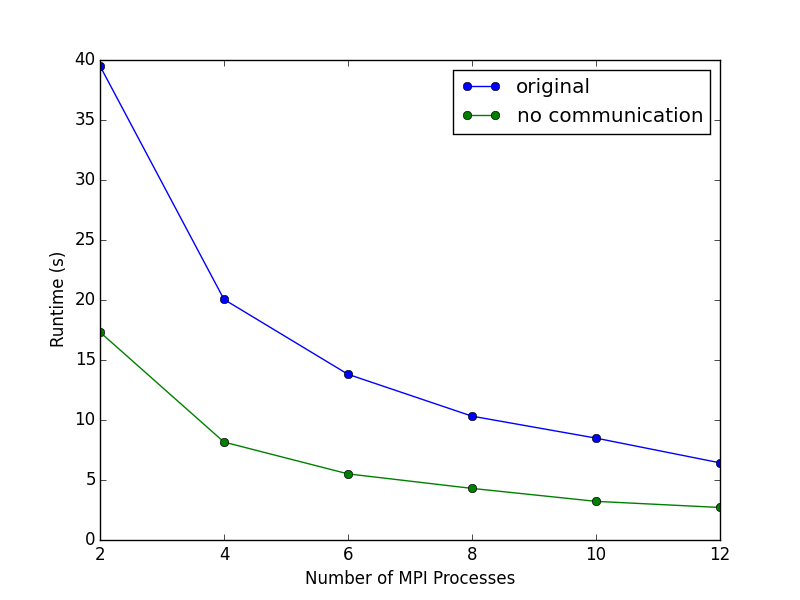
\includegraphics[width=0.6\textwidth]{../figures/nocomm.png}
\caption{Runtime for 20,000 elements both with and without communications within the DD iteration loop.}
\label{fig:nocomm}
\end{figure}

Reducing communication is difficult, because the simplicity of the interface solve does not justify overlapping computation with communication (each interface solve only computes {\it one} double precision number (since the solution for a two-element FE mesh with boundary conditions only involves solving for one constant). A smaller fraction of the runtime could be devoted to communication if more work could be allotted to the interface solve part. Currently, each process communicates with about 2 other processes just to compute one value. If the interface regions were wider, then both less DD iterations would be required and less communication per flop. However, as illustrated in the previous section, wider interface regions give incorrect results. With more time remaining, it would be possible to use small interface problems during the first phase of the solve until the solution becomes relatively smooth, and then transition to a wider interface to accelerate DD iterations. 

Fig. \ref{fig:scalingMPI} shows the (a) weak and (b) strong scaling obtained for the MPI parallelization. Scaling results are normalized relative to the runtime for the smallest recorded number of MPI processes used (in this case 2). For the weak scaling results, \(40000m\) elements are run for \(m\) MPI processes (i.e. the problem size is increased proportional to the number of processes). Results are shown for 1-3 MPI tasks per node. As can be seen, excellent weak scaling is obtained - by increasing the problem size proportional to the number of MPI processes, the speedup does not deviate from 1 (indicating that the algorithm behaves just as well as the problem size is scaled proportional to the number of processes). There also does not appear to be any clear optimal choice in the number of MPI tasks per node when judged using weak scaling. Strong scaling results are obtained using a fixed number of 100,000 elements and increasing the number of MPI processes. As can be seen, the strong scaling performance is excellent, and roughly increases as \(N^2\) due to the scaling of the CG method. When reporting the strong scaling for an algorithm that scales as \(N^2\), it is important to report the number of elements used, since the speedup will be even better for larger numbers of elements.

\begin{figure}[H]
        \centering
        \begin{subfigure}[b]{0.5\textwidth}
                \centering
                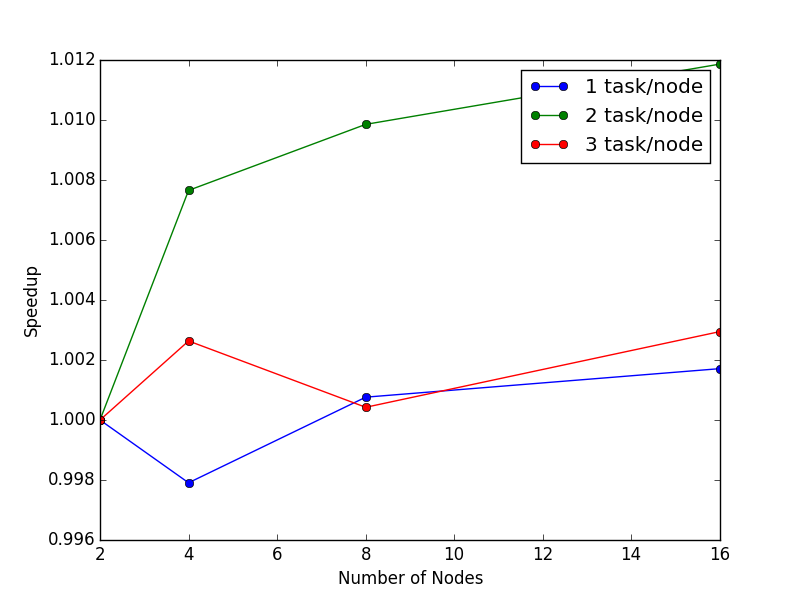
\includegraphics[width=\textwidth]{../figures/weak-mpi.png}
                \caption{Weak Scaling}
        \end{subfigure}%
                \begin{subfigure}[b]{0.5\textwidth}
                \centering
                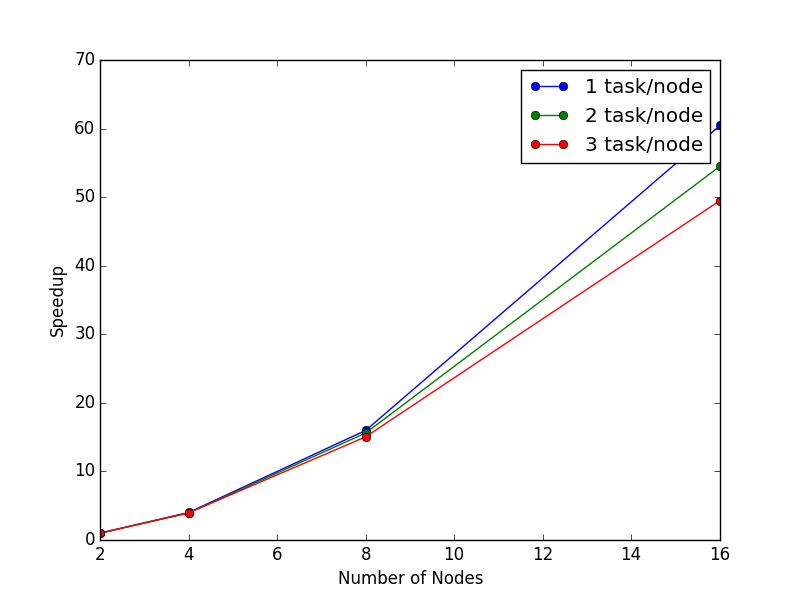
\includegraphics[width=\textwidth]{../figures/strong-mpi.png}
                \caption{Strong Scaling}
        \end{subfigure}%
\caption{Speedup as a function of the number of nodes with (a) the number of elements increase proportional to the number of processes and (b) the number of elements fixed at 100,000. Several lines show the performance for 1 to 3 MPI tasks per node.}
        \label{fig:scalingMPI}
\end{figure}

There are several ways in which the algorithm could be further improved to reduce communication and improve load balancing. As just discussed, wider interface problems would reduce the communication to computation ratio, and make the algorithm more computation-intensive. This would move the code to the ``right'' on the roofline model, and likely improve performance. A wider interface problem could be pursued without inducing errors in the solution if the wider interface is solved with recursive DD, in that more than one process solves each interface region. The extra communication required with this approach, however, might invalidate it for the simple 1-D domain investigated here, but could be useful in higher dimensions when the interface accounts for a smaller portion of the total domain.

Second, the DD algorithm is assumed converged when the relative difference in the interface boundary condition values changes little from one iteration to the next. While a {\it global} convergence such as this is required for Poisson problems where the problem is inherently global, it is possible to rewrite the algorithm such that convergence can occur for some processes, but not for others. For example, consider a five-process domain. Suppose that the initial guess was already fairly good in the domains belonging to processes 0 and 1, but very bad in the rest of the domain. The first two processes might converge in only a few iterations, but due to the global structure of my algorithm, they would need to continue iterating along with all of the other processes until {\it all} domains converge. Contrarily, a modification could be made to this algorithm such that processes that converge can be ``reallocated'' to the remaining, un-converged part of the domain. That is, once processes 0 and 1 converge, the remaining part of the domain could be re-divided amongst the five processes, and DD continue with different domains. Then, after a certain number of iterations, the original DD returned to to ensure that the solution in processes 0 and 1 is still accurate given further iterations in the rest of the domain. This algorithm might be called ``adaptive domain decomposition.'' 

\section{Conclusions}
I found this project topic to be very useful for my research, since DD is a common algorithm used to solve PDEs on high performance computers. This project revealed important aspects of DD, including:

\begin{enumerate}
\item While serial algorithms should be made to scale as \(\mathscr{O}(N)\) whenever possible, if poorer serial scaling is obtained, such as \(\mathscr{O}(N^2)\), then the impact of parallelization is even greater. Instead of linear speedup, quadratic, cubic, etc. speedup can be obtained. 
\item Parallel algorithms that introduce iterations into a non-iterative serial algorithm can potentially give much worse performance if the number of these iterations are large. For this project, using a good initial iterative solution guess (a similar effect to preconditioning) was used to obtain appropriately small numbers of DD iterations.
\item Finally, the decoupling of the decomposed domains has an important effect on the possible parallelization algorithms. In 1-D, both a master-slave approach and a shared-interface approach are possible, with the shared-interface approach achieving better load balancing. In higher dimensions, recursive DD could be used to shared solution to the interface problems among multiple MPI processes.
\end{enumerate}

And, I learned some practical code development wisdom as well, including:

\begin{enumerate}
\item Create a good Makefile early-on - I wasted a lot of time when working with Fortran modules by forgetting to compile one module that depended on others, and then struggling to realize why results were not as expected.
\item It is effective to first write a serial implementation that ``simulates'' parallelism by looping over the number of expected processes. This was a good starting point for parallelization, because it mostly involved removing loops and indexing by rank instead of loop iteration. In the assignments, we often started parallelizing without first developing a pseudo-parallel serial code, which I find to be more difficult.
\item Implement modern programming practices such as object-orientation and modularity as soon as possible. But, only you implement this, previous code that didn't use modules will likely be faster just to rewrite using the modules than to back-introduce modules into the code.
\end{enumerate}

\section{Running the Code}
Included in the {\tt zip} file submitted with this PDF are all of the source files, a Makefile for compilation, and an example job script that runs both the MPI code and the serial code for 20,000 elements for 2 to 24 MPI processes on a single node with domain length of 1, left boundary condition value of 2, and right boundary condition value of 3. To turn on output file writing to view the results, comment out the {\tt if (.false.)} clause towards the end of {\tt cmain.f90} (the MPI-parallelized version) and {\tt serial.f90} (the serial version). 















\end{document}
